\chapter{Implementierung einer grafischen Transceiver Applikation}
Ein als GNU Radio Flowgraph implementierter DAB/DAB+ Transceiver erfüllt funktionstechnisch alle notwendigen Anforderungen. Die Benutzerfreundlichkeit ist allerdings sehr eingeschränkt. Beispielsweise muss die Speicheradresse eines Kanals manuell aus der Konsole abgelesen werden, um sie im MSC Decoder anzugeben. Um die Benutzterfreundlichkeit zu erhöhen und den DAB/DAB+ Transceiver damit zu einer vollwertigen und ansprechenden Applikation werden zu lassen, wird eine Python Applikation mit grafischem Front-End implementiert, die mit den Namen \glqq \textit{DABstep}\grqq{} trägt.
\section{Klassenstruktur der Applikation}
Abb.~\ref{fig:class_diagramm} zeigt das Klassendiagramm der Applikation. Python Klassen sind durch abgerundete Ecken von den C++ Klassen unterscheidbar.

\begin{figure}[b!]
\begin{center}
\begin{tikzpicture}[node distance=1cm]
\tikzstyle{class_python}=[
    rectangle,
    rounded corners,
    draw=black,
    %text centered,
    anchor=north,
    text=black,
    text width=4cm]
\tikzstyle{class}=[
    rectangle,
    draw=black,
    %text centered,
    anchor=north,
    text=black,
    text width=4cm]

\node (dabstep) [class_python ,anchor = north, rectangle split, rectangle split parts=3]
    {
        \textbf{\centerline{\glqq DABstep\grqq{}}}
        \nodepart{second}-Frontend
        \nodepart{third}+show frontend()\newline+init transmitter()\newline +init receiver()\newline +play audio()\newline +set volume()\newline +get service info()\newline\centerline{...}
    };
\node (Frontend) [class_python, rectangle split, rectangle split parts=2, left =1.0cm of dabstep.north west, anchor = north east] 
    {
        \textbf{\centerline{Frontend}}
        \nodepart{second}-window\newline -tabs\newline -widgets\newline \centerline{...}
    };
\node (lookup tables) [class_python, rectangle split, rectangle split parts=2, right =1.0cm of dabstep.north east, anchor = north west, text width=2.7cm]
    {
        \textbf{\centerline{\begin{tabular}{cc}
Umsetzungs- \\
tabellen
\end{tabular}}}
    };
\node (usrp_tx) [class_python, rectangle split, rectangle split parts=3, below left= 1cm and 1cm of dabstep.south]
    {
        \textbf{\centerline{Transmitter}}
        \nodepart{second}-DAB Modus\newline -Frequenz\newline -MCI \& SI\newline -Audioquellen\newline -Ausgabegerät
        \nodepart{third}+run()\newline +set Volume()\newline\centerline{...}
    };
\node (usrp_rx) [class_python, rectangle split, rectangle split parts=3, below right= 1cm and 1cm of dabstep.south]
    {
        \textbf{\centerline{Receiver}}
        \nodepart{second}-DAB Modus\newline -Frequenz\newline -MCI eines Kanals\newline -Quelle (USRP/Datei)
        \nodepart{third}+run()\newline +get MCI()\newline +get SI()\newline +get SNR()\newline +set Volume()\newline\centerline{...}
    };
\node (fib_sink) [class, rectangle split, rectangle split parts=3, text width=3cm, below= of usrp_rx.260, anchor=north west]
    {
        \textbf{\centerline{FIB Senke}}
        \nodepart{third}+get MCI()\newline +get SI() \newline +get CRC passed()
    };
\node (dots3) [left=0.5cm of fib_sink]
    {
        $\cdots$
    };
\node (fic_encode) [class_python, rectangle split, rectangle split parts=2, text width=3cm, below= of usrp_tx]
    {
        \textbf{\centerline{FIC Encoder}}
        \nodepart{second}-DAB Modus
    };
\node (dots1) [right=0.5cm of fic_encode]
    {
        $\cdots$
    };
\node (fib_source) [class, rectangle split, rectangle split parts=2, text width=3cm, left= of fic_encode.north west, anchor = north east]
    {
        \textbf{\centerline{FIB Quelle}}
        \nodepart{second}-DAB Modus\newline -MCI \& SI\newline -DAB oder DAB+
    };
\node (xor) [class, rectangle split, rectangle split parts=2, text width=1.0cm, below= of fic_encode]
    {
        \textbf{\centerline{XOR}}
    };
\node (vector_source) [class, rectangle split, rectangle split parts=2, text width=3cm, below= 0.5cm of xor]
    {
        \textbf{\centerline{Vector Quelle}}
        \nodepart{second}-PRBS Sequenz
    };
\node (dots2) [right=0.5cm of vector_source]
    {
        $\cdots$
    };
\node (crc) [class, rectangle split, rectangle split parts=2, text width=3cm, left= 0.5cm of vector_source.north west, anchor = north east]
    {
        \textbf{\centerline{CRC}}
        \nodepart{second}-FIB Länge\newline -Gen. Polynom\newline -Initalstatus
    };
    
% arrows
\path [line] (Frontend.east) -- (dabstep.west|-Frontend);
\path [line] (lookup tables.west) -- (dabstep.east|-lookup tables);
\path [line] (dabstep.south) |- (usrp_tx.two east);
\path [line] (dabstep.south) |- (usrp_rx.two west);
\path [line] (usrp_rx.north) |- (dabstep.three east);
\path [line] (fib_source.north) -- ($(fib_source.north)+(0.0,0.5)$) -| (usrp_tx.240);
\path [line] (fib_sink.north) -- (usrp_rx.south-|fib_sink.north);
\path [line] (fic_encode.north) -- (usrp_tx.south);
\path [line] (xor.north) -- (fic_encode.south);
\path [line] (crc.north) -- ($(crc.north)+(0.0,0.5)$) -| (fic_encode.210);
\path [line] (vector_source.30) -- (fic_encode.south-|vector_source.30);
\path [line, dotted] (dots1) |- ($(usrp_tx.300)+(0.0,-0.5)$) -- (usrp_tx.300);
\path [line, dotted] (dots3) -- (usrp_rx.south-|dots3);
\path [line, dotted] (dots2) |- ($(fic_encode.south east)+(0.0,-0.5)$) -| (fic_encode.340);

\end{tikzpicture}
\end{center}
\caption{Klassendiagramm der DAB/DAB+ Transceiver Applikation}
\label{fig:class_diagramm}
\end{figure}

\subsection{Python main}
Die Python Klasse \glqq \textit{DABstep}\grqq{} stellt das Zentrum der Applikation aus Nutzersicht dar. Sie enthält alle Methoden, die den Nutzer mit der App interagieren lassen. Dazu gehören zum einen sog. Setter Methoden, die den Transceiver bzw. dessen C++ Blöcke steuern, also beispielsweise den DAB Empfänger starten oder die Lautstärke regeln. Zum anderen existieren sog. Getter Methoden, die Informationen aus den verschiedenen Blöcken des Flowgraphs extrahieren und zur Verfügung stellen. Ein wichtiges Beispiel hierfür sind die in der Applikation angezeigten Service Informationen, wie zum Beispiel eine Radiosenderliste. Zusätzlich existieren viele kleine Methoden, die für eine bessere Bedienbarkeit sorgen.

\subsection{Grafisches Frontend}
Die Informationen zum graphischen Design der Applikation liegen in einer separaten Klasse, dem sog. Frontend. Es beinhaltet alle Tabs, Steuerelemente (engl. Widgets), Beschriftungen, etc. und deren Anordnung im Anzeigefenster der Applikation. Für die Implementierung der graphischen Benutzeroberfläche (GUI) wird die Python Bibliothek PyQt4\footnote{Die aktuelle Nachfolgeversion PyQt5 verwendet Python3, was in GNU Radio noch nicht komplett unterstützt ist.} verwendet. Ein Großteil des Inhaltes dieser Klasse wurde mit dem Programm QtDesigner4 erzeugt.

\subsection{Umsetzungstabellen}
Eine dritte Python Klasse enthält alle Umsetzungstabellen (engl. lookup tables). Diese Umsetzungstabellen übersetzen die in Bits codierten Service Informationen wie zum Beispiel die Sprache oder das Land des DAB Ensembles in für Menschen lesbare Zeichenketten. Die Umsetzungstabellen sind in einem separaten Standarddokument der ETSI \cite{etsi:registered_tables} definiert.

\section{GNU Radio Flowgraphen}
Die funktionellen Kerne der Applikation sind die beiden GNU Radio Flowgraphen für den Transmitter und den Receiver. Sie enthalten die Definition, Instanzierung und Verbindung der einzelnen C++ Funktionalblöcke und bilden einen vollwertigen Transmitter bzw. Receiver. Im groben Aufbau entsprechen sie den bereits in vorherigen Kapiteln vorgestellten GNU Radio Flowgraphen aus Abb.~\ref{fig:grc_receiver} bzw. Abb.~\ref{fig:transmitter}. Abhängig von den Argumenten der Klasse werden die Flowgraphen aber individuell initialisiert. Zum Beispiel kann, je nach Konfiguration des Empfängers, eine Binärdatei oder Hardware als IQ Datenquelle dienen. Im Empfänger können ganze Zweige hinzukommen, wenn mehrere Audiostreams parallel gesendet werden.\\
Die Flowgraphen laufen in einem separaten Thread. Dies verhindert, dass die komplette Applikation eingefroren wird, wenn der Flowgraph zum Beispiel überlastet ist.

\subsubsection{GNU Radio Blöcke}
Die grundlegendste Klasse bilden die C++ Funktionalblöcke. Dazu gehören die in Abschn.~\ref{sec:imp_des_transmitters} und~\ref{sec:impl_des_receivers} beschriebenen Klassen des in diesem Projekt implementierten Moduls gr-dab, sowie einige grundlegende Blöcke aus anderen GNU Radio Modulen. Manche Gruppen von C++ Blöcken sind aus Gründen der Übersicht zu hierarchischen Python-Blöcken zusammengefasst.\\

Durch die genau definierte Funktion eines jeden Blocks und der hohen Flexibilität der GNU Radio Flowgraphen ist es möglich, nahezu die gesamte Datenverarbeitung und Entscheidungslogik innerhalb der Flowgraphen zu implementieren. Das hat den Vorteil, dass nur ein Minimum an Logik im Benutzerfrontend vorhanden sein muss.


\section{Datenfluss}
Ein Großteil des Datenflusses geschieht in den C++ Blöcken, die große Mengen an komplexen IQ Samples oder Bits mit hohen Raten verarbeiten müssen und diese über Ringbuffer an den jeweils nächsten Block übergeben. \\
Zusätzlich müssen aber auch Daten, wie zum Beispiel die MCI und SI, von den Datenverarbeitungsblöcken zur Benutzeroberfläche transportiert werden, um sie dort in einer strukturierten und für den Menschen gut lesbaren Form darzustellen. Bei diesem Datenstrom fallen geringe Datenmengen an und der Fokus liegt auf einer guten Strukturierung und Charakterisierung.
Eine geeignete Datenstruktur muss daher folgende Anforderungen erfüllen:
\begin{itemize}
\item Unterstützung \textbf{verschiedener Datentypen} (Zeichenketten für Sendernamen, Integer für Adressierungen, Boolean für Bitschalter)
\item \textbf{Flexible Struktur} in:
\begin{itemize}
\item Anzahl der Attribute (das Kanalinfo FIB enthält beispielsweise 5 Attribute, währende der Sendenamen FIB nur 2 Attribute beinhaltet)
\item Anzahl der Elemente (a priori ist nicht bekannt, wie viele Radiosender im empfangenen Ensemble enthalten sind, bzw. wie viel zusätzliche SI ausgestrahlt wird)
\end{itemize}
\item \textbf{Gute Lesbarkeit} für Menschen
\end{itemize}
Das Datenformat \ac{JSON} erfüllt diese Eigenschaften hinreichend und wird in dieser Arbeit für den Metadatenfluss zum graphischen Frontend verwendet.
\subsection{JSON}
Die grundlegenden Datenstrukturen des JSON Formats sind:
\begin{equation}
\begin{aligned}
object =& \biggl\{string : value,\;string : value,\; ...\biggl\} \\
array =& \biggl[value, \;value, \;...\biggl] \\
\text{mit} \; value \; \in& \; \{string,\; number,\; object,\; array,\; true,\; false,\; null\}
\end{aligned}
\end{equation}
Eine für die beschriebenen Anforderungen vorteilhafte Kombination von JSON Strukturen ist in Gl.~\ref{eq:json_example} beispielhaft für ein FIB mit Kanalinformationen dargestellt.
\begin{equation}
\label{eq:json_example}
\begin{aligned}
FIB = \biggl[
& \; \biggl \{ \text{\dq} ID \text{\dq} :4, \text{\dq} address \text{\dq} : 234, \text{\dq} size \text{\dq} : 84, \text{\dq} protection \text{\dq} : 2 \biggl \} \\
& \; \biggl\{\text{\dq}ID\text{\dq}:2,\text{\dq}address\text{\dq}:54,\text{\dq}size\text{\dq}:84,\text{\dq}protection\text{\dq}:3\biggl\} \\
& \; \biggl\{\text{\dq}ID\text{\dq}:3,\text{\dq}address\text{\dq}:138,\text{\dq}size\text{\dq}:96,\text{\dq}protection\text{\dq}:1\biggl\} \biggl]
\end{aligned}
\end{equation}
Das Array liefert die flexible Anzahl an Elementen und das Objekt bietet eine variable Anzahl an Attributen. Die Daten sind gut lesbar und werden genau in dieser Form als Zeichenkette in den jeweiligen Blöcken, ein Großteil davon in der FIC Senke, generiert. Diese können dann von der Receiver Klasse über eine Getter Funktion abgefragt und an die Klasse \textit{DABstep} weitergeleitet werden wo sie an entsprechender Stelle angezeigt werden. Das Lesen der Daten in DABstep gestaltet sich besonders intuitiv, da ein JSON Array als Python Array und ein JSON Objekt als Python Dictionary interpretiert werden kann. Die einzige Datenverarbeitung, die an dieser Stelle vom Benutzerfrontend durchgeführt werden muss, ist das Lesen, Sortieren und Anzeigen der JSON Objekte.

\section{Grafischer Aufbau}
Neben der Funktionalität steht bei der grafischen Applikation \textit{DABstep} vor allem auch die Benutzerfreundlichkeit im Mittelpunkt. Die Applikation soll von Laien intuitiv bedienbar sein und übersichtlich bleiben. Das Programm ist in Empfänger und Sender aufgeteilt, welche über zwei Tabs erreichbar sind. Abb.~\ref{fig:GUI_receiver} zeigt die Empfängerseite.
\begin{figure}[htb]
\centering
  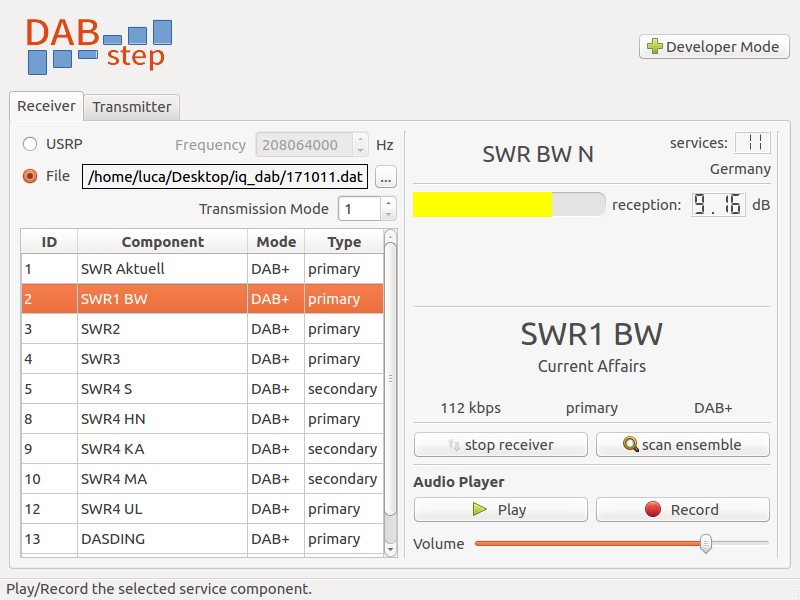
\includegraphics[width=\textwidth]{figures/GUI_receiver.png}
	\caption{DABstep im Empfängermodus}
	\label{fig:GUI_receiver}
\end{figure}
Die räumliche Aufteilung ist dem sequentiellen Ablauf einer Empfangssituation nachempfunden:
\begin{enumerate}
\item \textbf{Initiale Einstellungen}: Wahl der Quelle, DAB Modus und Mittenfrequenz.
\item \textbf{Senderliste}: Anzeige und Auswahlfeld der DAB Sender.
\item \textbf{Informationen}: Anzeige von zusätzlichen Informationen über das empfangene DAB Ensemble und den ausgewählten Sender.
\item \textbf{Audio}: Kontrolle über die abgespielte Musik, zum Beispiel Lautstärkeregelung oder Aufnahmefunktion.
\end{enumerate}
\\
Während die Empfängerseite hauptsächlich Informationen anzeigt, liegt der Schwerpunkt bei der Senderseite auf dem Schreiben von Informationen für das zu sendende DAB Ensemble. Um die Bedienfreundlichkeit zu bewahren, wurde die Aufteilung im Sender von der funktionalen Aufteilung analog zum Empfänger gestaltet. Abb.~\ref{fig:GUI_transmitter} zeigt die GUI im Sendemodus.
Die Wahl zwischen Hardware und Binärdatei ist auch im Sendemodus vorhanden und definiert in diesem Fall die Art der Senke. Die Informationen über die einzelnen Radiosender können über die Eingabeformulare individuell eingestellt werden. Es ist dabei auch möglich in einem Ensemble DAB und DAB+ Kanäle zu mischen. Als Audioquelle gibt es neben Audiodateien auch die Möglichkeit, die lokale Soundkarte mit einem Mikrofon zu nutzen.
Im rechten oberen Bereich sind, wie im Empfänger, die Ensemble Informationen platziert. Durch das Erhöhen der Anzahl der Kanäle wird die Spalte mit den Informationen zu den einzelnen Kanälen auf der linken Seite automatisch um eine Komponente für den neuen Kanal ergänzt. Die Audioeinstellungen befinden sich auch hier im rechten unteren Bereich der Oberfläche. Der Benutzer muss den Kanal, den er hören will, auswählen, da er logischerweise nicht alle Kanäle des DAB Ensembles gleichzeitig hören kann.

\begin{figure}[htb]
\centering
  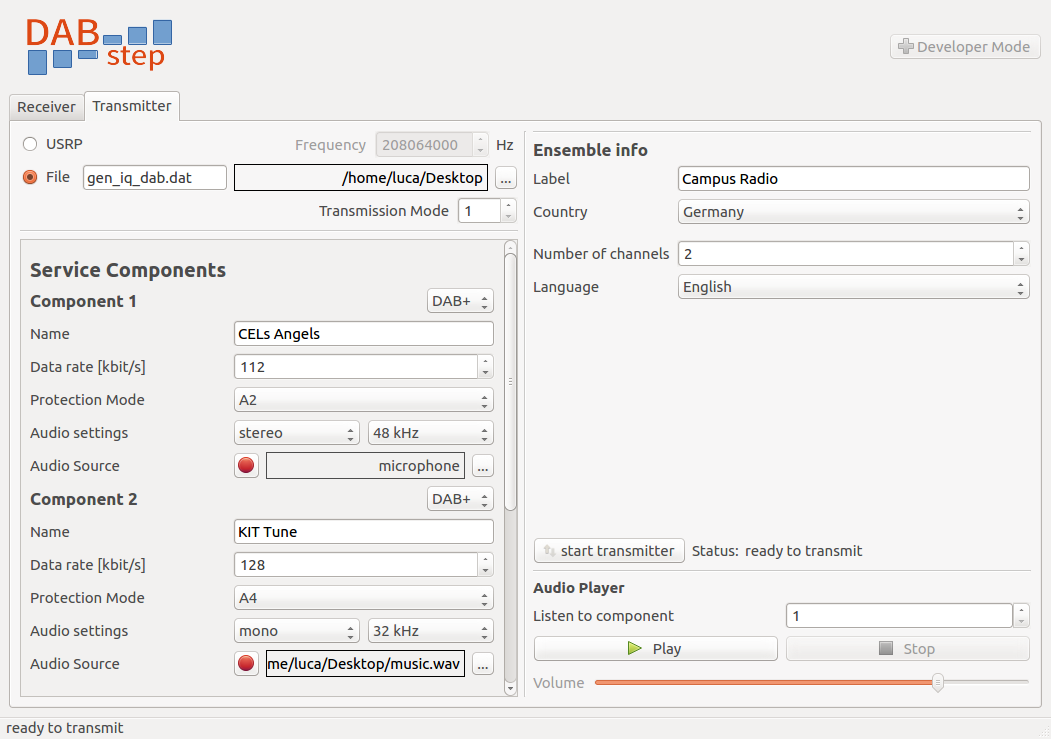
\includegraphics[width=\textwidth]{figures/GUI_transmitter.png}
	\caption{DABstep im Sendemodus}
	\label{fig:GUI_transmitter}
\end{figure}

\subsubsection{Entwicklermodus}
Eine Besonderheit stellt der Entwickler-Modus dar, welcher in der Empfängerseite über das \glqq +\grqq{}  Symbol in der oberen rechten Ecke erreichbar ist. Dieser erweitert die GUI um einige technische Anzeigen (siehe Abb.~\ref{fig:GUI_dev_mode}). 

\begin{figure}[htb]
\centering
  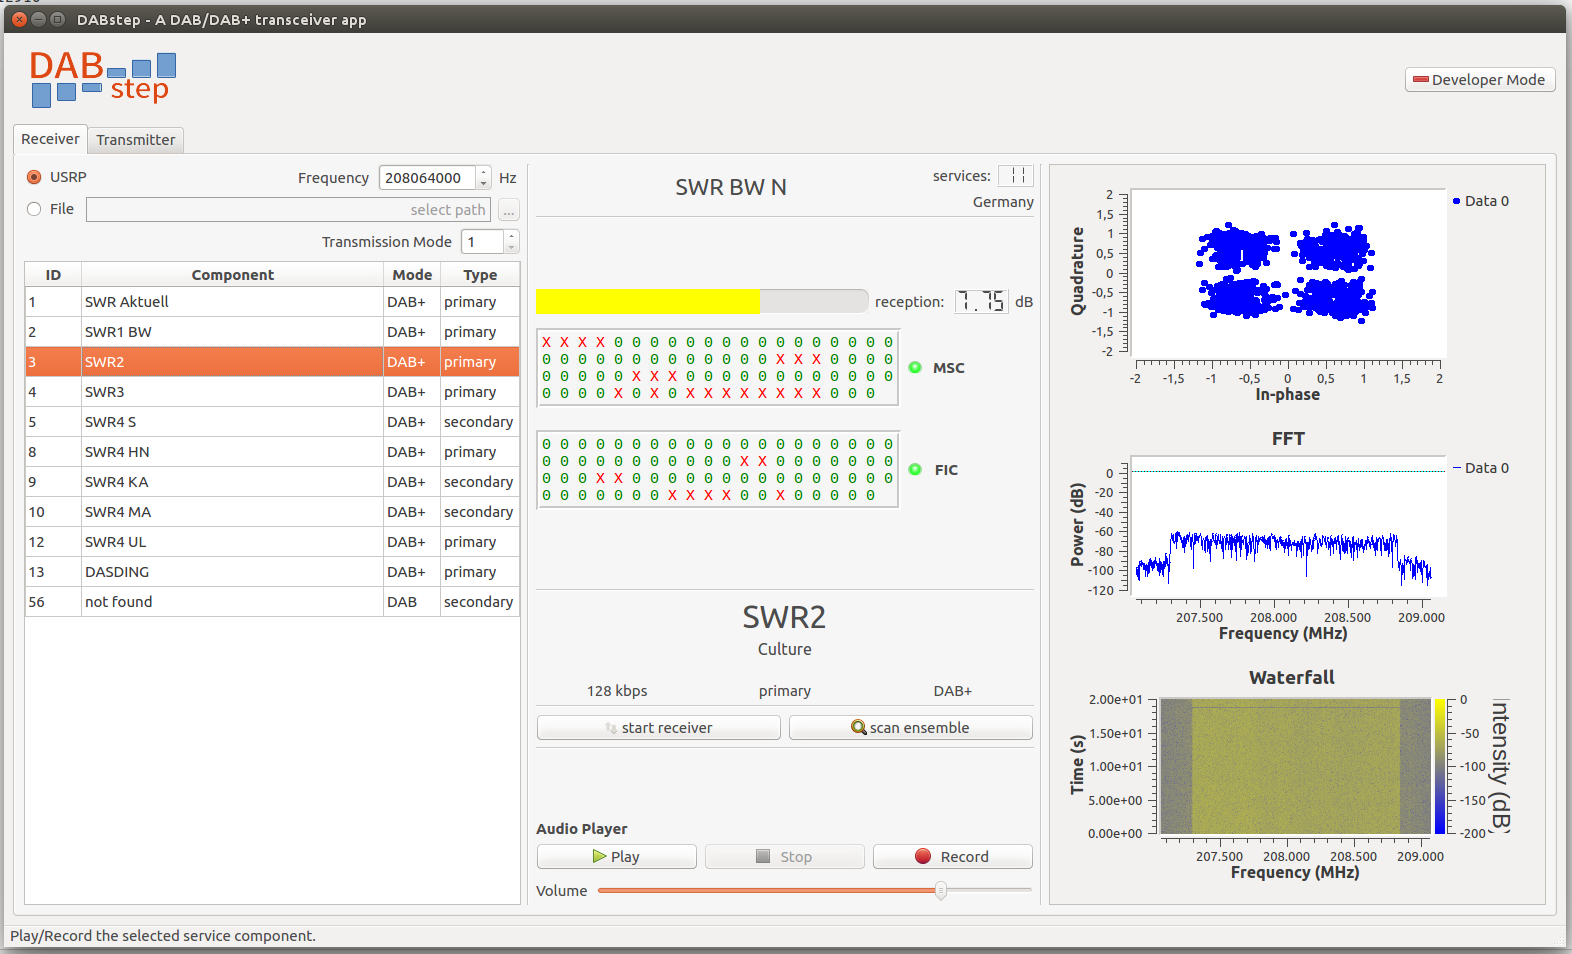
\includegraphics[width=\textwidth]{figures/GUI_dev_mode.png}
	\caption{DABstep im Entwicklermodus}
	\label{fig:GUI_dev_mode}
\end{figure}

Eine Anzeige für die Fehlerrate, getrennt für FIC und MSC, stellt das Ergebnis des CRC checks der FIBs bzw. des Firecode Checks für die Audio Frames dar. Die rechte Spalte ergänzt die GUI um ein Konstellationsdiagramm, eine FFT Anzeige und einen Wasserfall Plot. Die drei Widgets wurden dabei aus dem GNU Radio Modul \textit{gr-qtgui} \cite{repo:gr-qtgui} übernommen, in den Flowgraph eingebaut und beim Öffnen des Entwicklermodus an die GUI als Objekte übergeben.